

\section{Platinenentwurf}
In Anbetracht der Tatsache, dass die Realisierung der 8 Klänge aufgrund von 3 verschiedenen Schaltungstypen theoretisch den Einsatz individueller Platinen erfordern würde, wurde ein effizienterer Ansatz gewählt. Anstelle der Produktion von drei separaten Platinen, was mit erheblichen Kosten verbunden wäre, wurden die verschiedenen Platinendesigns integriert, um eine einheitliche Platine zu schaffen, die es ermöglicht, alle individuellen Klänge durch die Anpassung der Bauteilbestückung zu erzeugen.

\begin{figure}[h]
    \centering
    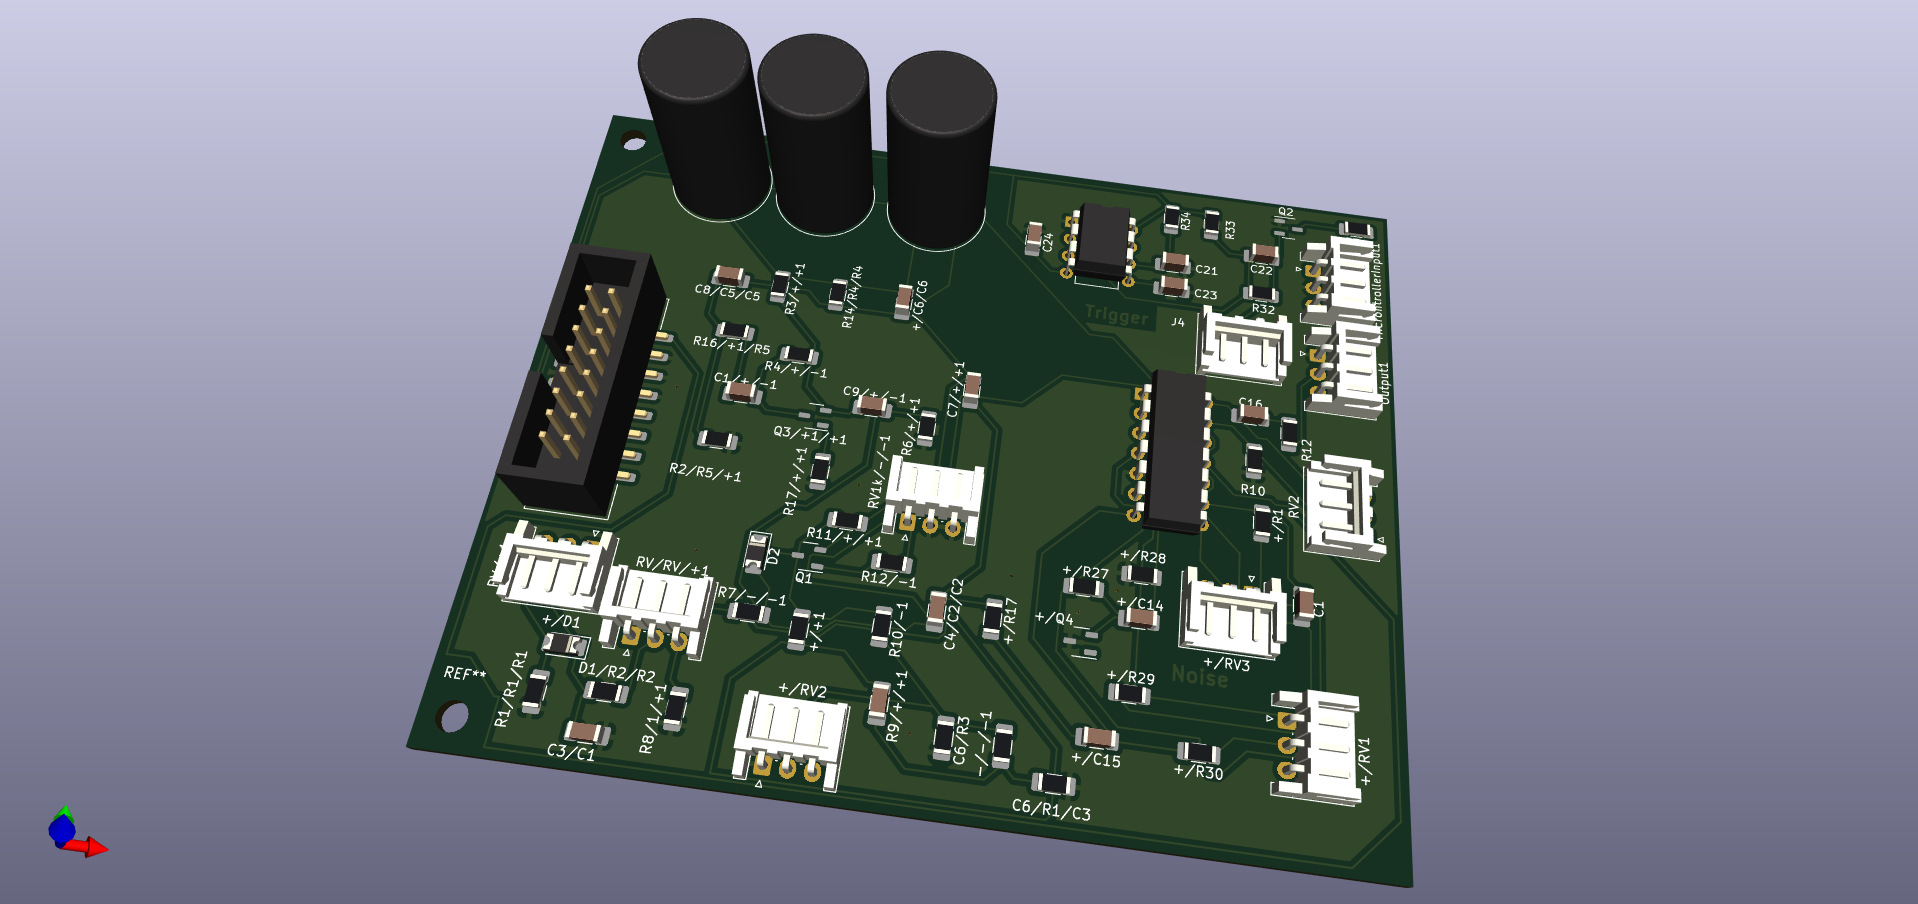
\includegraphics[width=0.8\textwidth]{Images/KiKAD_Endplatine_V2.png}
    \caption[Leiterplattenentwurf]{3D-Ansicht der Leiterplatte}
    \label{fig:3D-Ansicht der Leiterplatte}
    \source{KiCad 3D-Ansicht}
\end{figure}

Die Planung und Gestaltung der Platine erfolgte mithilfe von KiCad, einem Open-Source Programm für die Entwicklung von Leiterplattenentwürfen. In Fällen, in denen bereits vorhandene Bauteile wie 3-Pin-Anschlüsse zur Verfügung standen, wurden diese wiederverwendet und entsprechend in das Platinendesign integriert
